\subsubsection{Reporting}
Reports should be generated based on the data selection and then be exported to a known format.\\ \\
Formats include:
\begin{itemize}
	\item PDF
	\item CSV
	\item HTML\\
\end{itemize}
\textbf{Pre-Conditions}
\begin{itemize}
	\item The user must be logged into UPRM to generate reports.
	\item The user must have the right privileges to be able to export the specific data.\\
\end{itemize}
\textbf{Post-Conditions}
\begin{itemize}
	\item A report in the specified format should open or be saved on the local computer of the user.\\
\end{itemize}
\textbf{Reporting Use Case Diagram:}\\
\centerline{\fbox{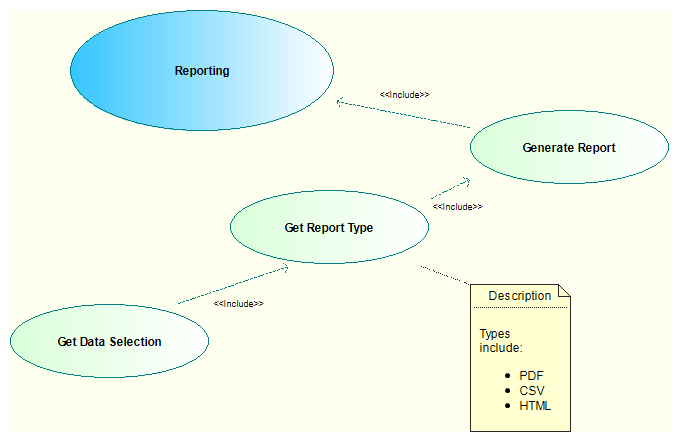
\includegraphics[width=\linewidth]{reporting/Reporting}}}